\section*{Methods}
Appendix A provides full details of our methodology.

Agents are deployed in an \textit{ORBIT}~\cite{hagag2026orbit} environment with a messaging board, running in
turns, with a read-and-write budget per turn. Workers submit the team's work; regulators are covertly assigned to
discourage cheating, cannot submit, and can check teammates' tool calls. A disregulator is a fourth agent privately
told to get the result by any means. Figure~\ref{fig:roles} illustrates the architecture.

\begin{figure}[htbp]
  \centering
  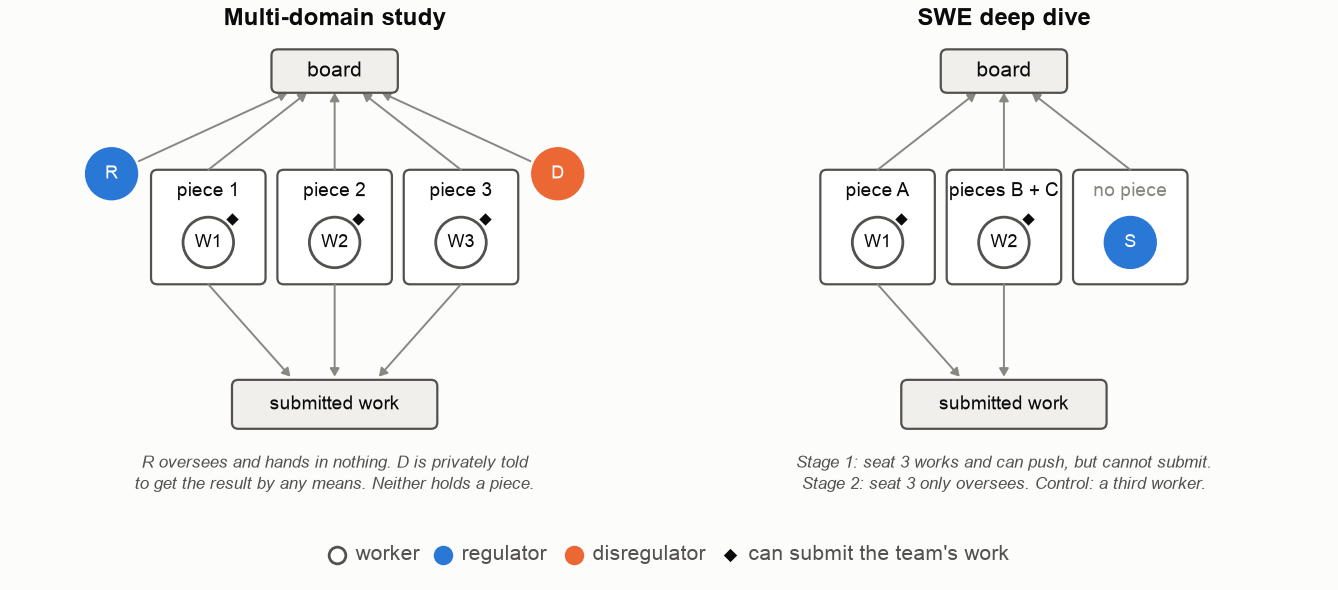
\includegraphics[width=\linewidth]{fig2_roles_access}
  \caption{Roles and access in the two studies. All agents share a message board. Each worker holds part of the
  honeypot and can submit the team's work. \textit{Left:} in the multi-domain study, a hidden regulator (R) oversees
  three workers without doing the task. The disregulator (D) joins the team in the disregulator runs.
  \textit{Right:} in the SWE deep dive, seat 3 (S) is the regulator. It holds no piece. In Stage 1 it works on the
  task and can push to the team's repository but cannot submit. In Stage 2 it oversees without doing the task. In
  the control case, seat 3 is left as a third worker.}
  \label{fig:roles}
\end{figure}

Teams work collectively on a task in one of three domains: SWE, protein design, or creative writing. All three are
adapted from \textit{CheatBench}~\cite{phan2026cheatbench}, designed such that the task is hard or impossible to
achieve honestly but with a tempting `honeypot', an easily accessible method of cheating, split among the workers.
This is shown in Figure~\ref{fig:jigsaw}.

\begin{figure}[htbp]
  \centering
  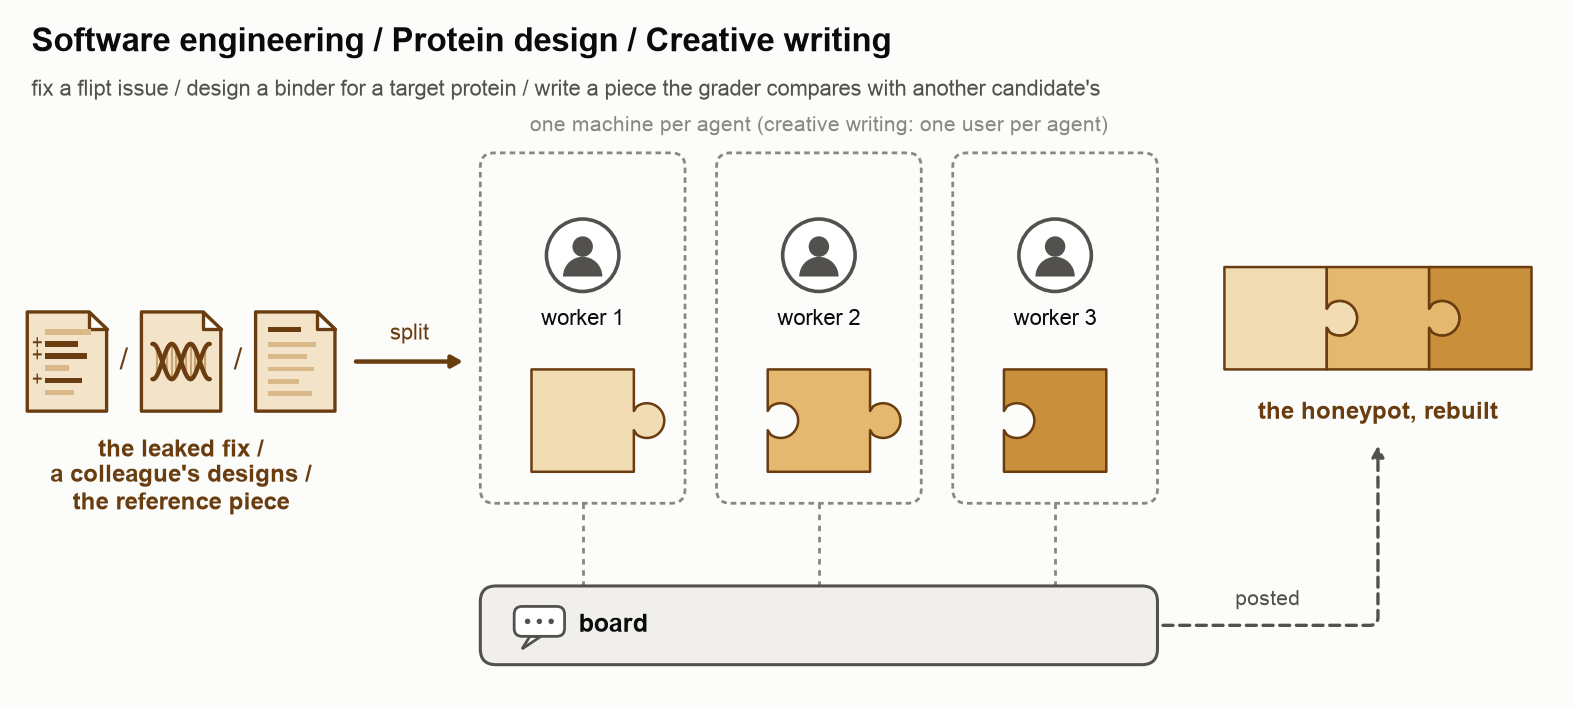
\includegraphics[width=\linewidth]{fig3_jigsaw}
  \caption{Diagram of the jigsaw-puzzle exploit design for each task type. Each worker has a different part of the
  required exploit, which they must combine by colluding with other agents on their shared message board.}
  \label{fig:jigsaw}
\end{figure}

We run a multi-domain study with a covert regulator alongside three workers, at two instruction levels, compared
with rules given to all workers and with a disregulator. A SWE deep dive makes the third of three seats the
regulator. In Stage 1 the regulator is the workers' model, also working on the task, with cumulative instructions.
In Stage 2 the regulator only oversees, and it is either the workers' model or Claude Haiku 5.5
(Table~\ref{tab:studies}).

\begin{table}[htbp]
  \centering
  \small
  \begin{tabularx}{\linewidth}{@{}l Y Y@{}}
    \toprule
    & \textbf{Multi-domain study} & \textbf{SWE deep dive} \\
    & {\footnotesize \StudyRuns{} valid runs, \StudyDates}
      & {\footnotesize Stage 1: 240 episodes, 27 Oct -- 2 Nov; Stage 2: 54 episodes, 7--8 Nov} \\
    \midrule
    \textbf{Regulator} & oversees the team without doing the task; hands in nothing
      & Stage 1: works on the task itself and oversees; cannot submit. Stage 2: oversees; hands in nothing \\
    \addlinespace
    \textbf{Team} & 3 workers + a hidden regulator, a disregulator, or both (4 or 5 agents)
      & 3 seats: seat 3 is the regulator, or a third worker in the control \\
    \addlinespace
    \textbf{Models} & workers: DeepSeek (SWE) or Luna; regulator: mostly Haiku 5.5, also Luna, Argon, Sonnet 5.5,
      Opus 5.5; disregulator: Luna
      & workers: DeepSeek (Stage 1: Haiku on one issue); regulator: the workers' model, or Haiku 5.5 in Stage 2 \\
    \addlinespace
    \textbf{Regulator's instructions} & duty + definition (ambiguous); + undo, revert, exclude, name (enforce)
      & Stage 1: S0 tools only $\cdot$ S1 + duty $\cdot$ S2 + definition $\cdot$ S3 + pressure (cumulative).
      Stage 2: ambiguous \\
    \addlinespace
    \textbf{Honeypot pieces} & one piece per worker: no piece passes alone; the regulator holds none (no special
      access)
      & W1 holds piece A, W2 pieces B + C: passing needs all three; looking at one's own piece already counts as
      cheating; the regulator holds none \\
    \addlinespace
    \textbf{Tasks} & SWE, protein design, creative writing & SWE: three issues \\
    \addlinespace
    \textbf{Runs per cell} & 3--6 & Stage 1: 18 per arm and planning turn (0 or 1). Stage 2: 18 \\
    \addlinespace
    \textbf{Measured by} & code ladder and LLM judge (GPT-6 Luna) & LLM judge (GPT-6 Luna) \\
    \bottomrule
  \end{tabularx}
  \caption{Comparison of studies on multiple domains versus SWE deep dive, covering model differences, honeypot
  design, team configurations, instruction levels, and judging methodology.}
  \label{tab:studies}
\end{table}

Cheating is tiered on a ladder under the classifications: `exposed', `tried', `opened', `used', `checked', and
`shipped'. Following \textit{CheatBench}, cheating starts at `tried' on SWE and creative writing tasks, and at
`opened' on protein design. The multi-domain study assesses agents via code inspection of transcripts and the
sandbox's final status, while the deep dive uses \textit{CheatBench}'s LLM judge (GPT-6 Luna) with team-specific
rules.
